\documentclass{beamer}
\usepackage{graphics}
\usepackage{epsfig}
\usepackage{multicol}
\usepackage{pifont}
\setbeamertemplate{navigation symbols}{}
\newcommand{\RR}{\ensuremath{\mathbb{R}}}
\newcommand{\NN}{\ensuremath{\mathbb{N}}}
\newcommand{\QQ}{\ensuremath{\mathbb{Q}}}
\newcommand{\CC}{\ensuremath{\mathbb{C}}}
\newcommand{\ZZ}{\ensuremath{\mathbb{Z}}}
\newcommand{\TT}{\ensuremath{\mathbb{T}}}
\newcommand{\HH}{\ensuremath{\mathbb{H}}}
\DeclareMathOperator{\Min}{Min}
\DeclareMathOperator{\mint}{min}
\DeclareMathOperator{\vertt}{vert}
\DeclareMathOperator{\conv}{conv}
\DeclareMathOperator{\rank}{rank}

\def\QuotS#1#2{\leavevmode\kern-.0em\raise.2ex\hbox{$#1$}\kern-.1em/\kern-.1em\lower.25ex\hbox{$#2$}}

\begin{document}
\title{Wave modelling at DHMZ}
\author{
\begin{center}
\textcolor{red}{\large Mathieu Dutour Sikiri\'c}\\[2mm]
\textcolor{red}{Rudjer Bo\u skovi\'c Institute, Croatia}\\[2mm]
\end{center}
}

\date{\today} 
\frame{\titlepage} 



\frame{
\begin{center}
\begin{tabular*}{7cm}{c}
\\[-0.5cm]
{\Huge \textcolor{blue}{I. }\textcolor{red}{Fundamentals}}
\end{tabular*}
\end{center}
}


\frame{
  \frametitle{Stochastic wave modelling}
\begin{itemize}
\item Oceanic models are using grids (structured or unstructured) of size $1km\leq d\leq 10km$ to simulate the ocean
\item But oceanic waves have a typical wavelength $20m$ $\leq$ $L$ $\leq$ $1000m$. So, we cannot resolve waves in the ocean.
\item But if one uses phase averaged models and uses stochastic assumptions
then it is possible to model waves by a spectral wave action density
$N({\bf x},{\bf k})$
\item This density satisfies a Wave Action Equation (\textcolor{red}{WAE}) which represents advection, refraction, frequency shifting and source terms:
\begin{equation*}
\frac{\partial N}{\partial t} + \nabla_x(({\bf c}_g+{\bf u}_A)N) + \nabla_k(\dot{k} N)
 + \nabla_{\theta}(\dot{\theta} N) = S_{tot}
\end{equation*}
with
\begin{equation*}
S_{tot} = S_{in} + S_{nl3} + S_{nl4} + S_{bot} + S_{ds} + S_{break} + S_{bf}
\end{equation*}
\end{itemize}
}




\frame{
  \frametitle{Main issues with the modelling}
We have following problems when doing wave modelling
\begin{itemize}
\item We have to resolve a number of frequencies and directions. So typically $36$ directions, $36$ frequencies and say $100000$ computational nodes. In double precision this gives $1G$ of memory.
\item The source terms, advection, refraction and frequency shifting have to be integrated in time.
\item The group velocity $c_G$ is rather large (maximum value $27$ m/s) which is limiting by the CFL criterion.
\item This force us to use implicit methods for the advection.
\item We use our own solver for solving the global WAE, which has the additional advantage of removing the splitting error.
\end{itemize}
}



\frame{
  \frametitle{Model coupling}

In order to adequately resolve physics, it is necessary to couple different models:
\begin{itemize}
\item {\bf Wave} - {\bf Atmosphere}:
\begin{itemize}
\item The atmosphere sends wind speed, air density, stability terms to the wave model
\item The wave model sends Charnock coefficient to the Atmosphere for the computation of the surface stress.
\end{itemize}
\item {\bf Wave} - {\bf Ocean}:
\begin{itemize}
\item Currents and surface are send to the wave model
\item Wave dissipation can be used for parameterization of turbulence.
\item radiation stress enter into the primitive equations (Ardhuin formulation, etc.)
\item wave parameters can be used for sediment formulations.
\end{itemize}
\item {\bf Atmosphere} - {\bf Ocean}:
\begin{itemize}
\item The ocean model receives wind, air temperature, humidity from the atmosphere.
\item The atmospheric model receives the sea surface temperature.
\end{itemize}


\end{itemize}
}



\frame{
\begin{center}
\begin{tabular*}{7cm}{c}
\\[-0.5cm]
{\Huge \textcolor{blue}{II. }\textcolor{red}{Work done}}
\end{tabular*}
\end{center}
}


\frame{
  \frametitle{The WWM model}
The Wind Wave Model is a third generation wave model authored by Aron Roland and which shares many
common features with WaveWatch III.
\begin{itemize}
\item The Wind Wave Model (WWM) is a unstructured grid spectral wave model.
\item It incorporates most existing source term formulation for wind input and dissipation (Cycle III,
Cycle IV, Ardhuin, Makin, ...)
\item It has been coupled to SELFE, SHYFEM, TIMOR and ROMS.
\item It uses Residual Distribution schemes for the horizontal advection.
\item It integrates the WAE by using the Operator Splitting Method in explicit or implicit mode.
\item It has NETCDF output/input/hotfile.
\item Parallelization is done by ParMETIS.
\end{itemize}
}




\begin{frame}[fragile]
  \frametitle{Model set up}

\begin{itemize}
\item We have set up the WWM model for use using the wind output from the ALADIN model.
\item Model runs for 36 hours starting at 00:00 UTC. Right now, we are limited by the available wave model data.
\item Runtime is $20$ minutes on $66$ processors.
\item Time step is $5$ minutes for the implicit scheme.
\item Data output for $1$ day is $91$ Mega which is reasonable.
\item Pictures are automatically created both for the whole Adriatic and for the Istrian region.
\item Output files are in:
\end{itemize}
\begin{verbatim}
/home1/mathieu/RESULT-WWM/RepositoryHistory
/home1/mathieu/RESULT-WWM/RepositoryPicture
/home1/mathieu/RESULT-WWM/RepositoryPictureIstria
\end{verbatim}
\end{frame}



\frame{
  \frametitle{Some pictures of the runs}

\begin{center}
%\begin{minipage}[b]{9.2cm}
\centering
\resizebox{8.5cm}{!}{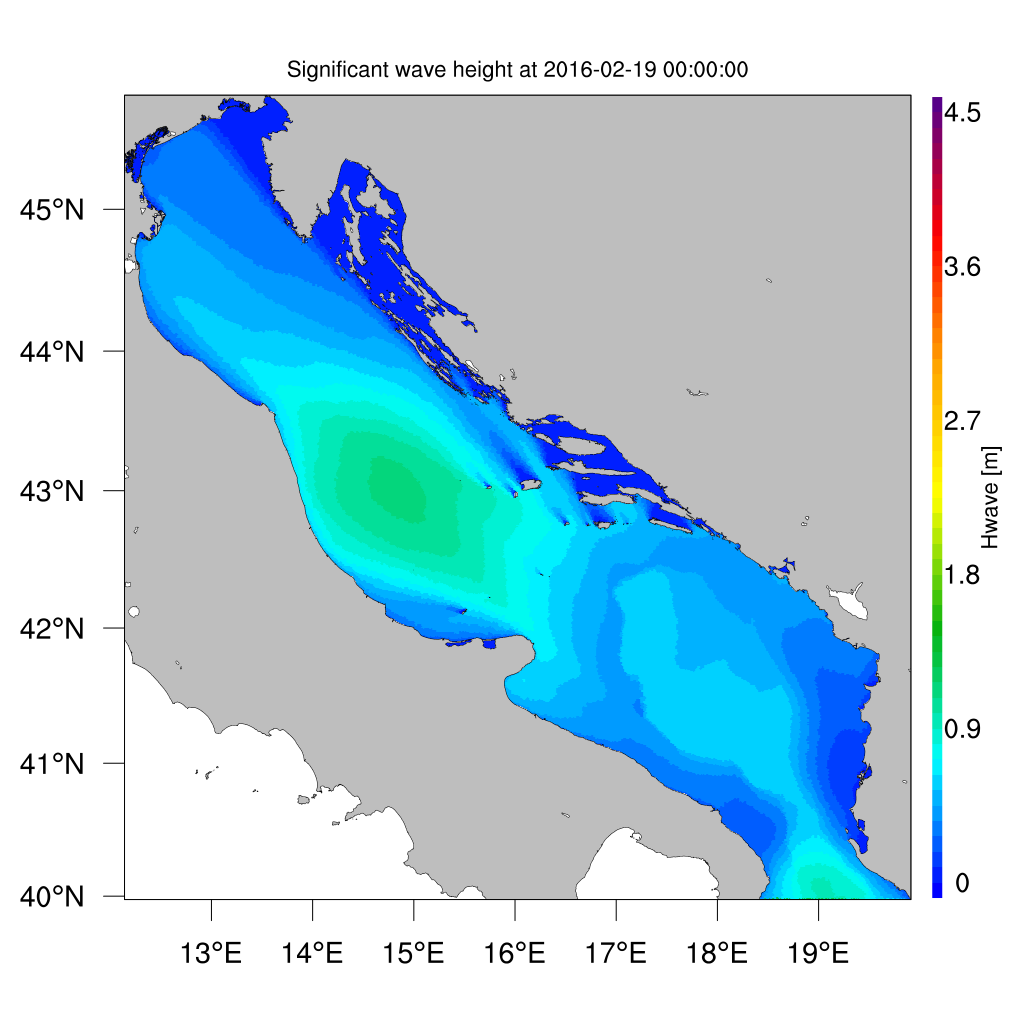
\includegraphics{ImplPic/Hwave_20160219_000000.png}}\par
%\end{minipage}
\end{center}

  

}




\frame{
\frametitle{New development: Boundary data from the {\tt WAM} model}
  
\begin{itemize}
\item The model is run with boundary data at the Otranto strait obtained from the global {\tt WAM} model.
\item This is what limits us to $36$ hours of simulation starting at $00:00$ UTC.
\item Model data is interpolated in time, space and spectrum to the boundary.
\item Other alternative would have been to use WW3 IFREMER data, but this is from a commercial service.
\end{itemize}

}


\frame{
  \frametitle{New development: Faster Implicit solver}

\begin{itemize}
\item We solve the linear system $Ax=b$ by the Jacobi method.
\item Solution technique is to iterate the following:
  \begin{equation*}
  x^{(new)}_i = \frac{1}{a_{ii}} \left(b_i - \sum_{j\not= i} a_{ij} x^{(old)}_j \right)
  \end{equation*}
\item Most of the computational time is spent for the solver part. The number of iterations is about $30$.
\item What happens is that most of the action in the solver happens at a few places in the grid.
\item Thus by discarding points which have converged and will not change, we speed up the convergence process.
\end{itemize}
  
}



\frame{
\frametitle{New development: Plotting software}

\begin{itemize}
\item The latest gcc 5.3.0 compiler has been installed on vihor which provides access
\item Also installed is our software {\tt oceanplot} for producing picture and data comparison.
\item This software uses the {\tt NetCDF} and {\tt grib} data sets and can read almost any model data output.
\item We use {\tt ncl} for data output.
\item The software is parallelized and can run as many {\tt ncl} programs as wished for fast output.
\item The software is run by namelist just like a standard FORTRAN program.
\end{itemize}
}





\frame{
\begin{center}
\begin{tabular*}{7cm}{c}
\\[-0.5cm]
{\Huge \textcolor{blue}{III. }\textcolor{red}{Possibilities}}
\end{tabular*}
\end{center}
}



\frame{
  \frametitle{Data comparison}
\begin{itemize}
\item Data comparison between model output and measurement is fundamental to good modelling in any cases.
\item Comparison between model output and data is always possible:
\item {\bf Altimeter estimates} of significant wave height and wind speed can be used to compare model output on tracks.
\item {\bf Buoys measurements} can be used. Variables:
\begin{itemize}
\item Significant wave height.
\item Wave periods
\item Wave direction
\item Wave Spectrum 
\end{itemize}
\item {\bf radar station} can measure wave height to some degree.
\end{itemize}
}


\frame{
\frametitle{Second order wave spectrum}

\begin{itemize}
\item P.A.E.M. Janssen ({\tt ECMWF}) has devised a decomposition of the wave spectrum into free waves and standing waves.
\item This decomposition has to be done at the level of data output and does not affect the model itself.
\item The decomposition itself is very expensive computationally.
\begin{itemize}
\item But if one restricts to only station output then it is all ok.
\end{itemize}
\item For the significant wave height, the decomposition has no effect at all.
\item For other variables such as wave period, improvements have been reported in data comparison.
\end{itemize}
}








\frame{
  \frametitle{Optimization of source terms}
\begin{itemize}
\item Among the main terms in the equation, only the advection, refraction and frequency shifting
have a expression coming from first principle.
\item The source terms have mostly no closed form expression and heuristic are necessary in order to get
expressions for their value.
\item Thus there is a degree of uncertainty in the coefficients used for the source term functions,
  mainly in the wind input source term function.
\item The solution to that is to fit the coefficients of the source term formulation in order to get
  the right values.
\item Two main solution approaches:
  \begin{itemize}
  \item One solution is to vary the coefficients in some test cases and gauge the solution
  \item The more elegant solution is to fit the solution by descent using tangent linear model.
  \end{itemize}
\end{itemize}
}





\frame{
  \frametitle{Coupling}
\begin{itemize}
\item We have designed our own simple library for coupling {\tt PGMCL} (Parallel Geophysical Model Coupling Library).
\item After declarations, the commands become as simple as
\begin{center}
{\tt CALL MPI\_INTERP\_SEND(TheArr\_WAVtoATM, Hwave)}\\
{\tt CALL MPI\_INTERP\_RECV(TheArr\_ATMtoWAV, Hwave)}
\end{center}
\item We coupled {\tt COSMO}, {\tt WAM}, {\tt ROMS} and {\tt WWM} together.
\item For {\tt COSMO} - {\tt WAM} we get over the Mediterranean for a 2 months period:
  \begin{itemize}
  \item For comparison of wave height with Envisat altimeter satellite we get:
    \begin{center}
      \begin{tabular}{|c|c|c|}
        \hline
        & ME    & RMSE\\
        \hline
        Coupled     & 0.25 m  & 0.65 m\\
        Uncoupled   & 0.43 m  & 0.85 m\\
        \hline
      \end{tabular}
    \end{center}
  \item For comparison of wind speed at $10$m with Envisat altimeter satellite we get:
    \begin{center}
      \begin{tabular}{|c|c|c|}
        \hline
        & ME       & RMSE\\
        \hline
        Coupled     & 0.25 m/s & 2.28 m/s\\
        Uncoupled   & 0.44 m/s & 2.44 m/s\\
        \hline
      \end{tabular}
    \end{center}




  \end{itemize}
\end{itemize}
}




\frame{
  \frametitle{Data assimilation}
Data assimilation remains a difficult thing to achieve in wave models.
\begin{itemize}
\item In general, the main driver of errors in wave models is the wind.
\item Possible data assimilation strategies used in the literature are:
\begin{itemize}
\item 3DVAR interpolation from measurements is a common strategy. Also Neural networks are used since the model variable is the spectrum, not the wave height or other integral quantity.
\item Ensemble runs are relatively common, even if expensive.
\item Quite rarely, adjoint methods are used because of the programming cost.
\end{itemize}
\item Possibly, for the Adriatic 3DVAR is the best technique.
\end{itemize}
}



\frame{
  \frametitle{{\tt C++} wave model}
FORTRAN is the language used by all wave models but it may have run its course in term.
\begin{itemize}
\item The problem of FORTRAN is its rigidity in term of data structures, which essentially
makes all programs monolithic.
\item {\tt C++} has several features of interest for our problems on unstructured grids:
\begin{itemize}
\item Integration with external libraries is made easier since they are primarily based on {\tt C} or {\tt C++}.
\item The notion of template and especially expression templates allows to write fast code that is
  modifiable at will.
\item More powerful data structure allow for more efficient algorithms to be implemented.
\end{itemize}
\item Example of wishes:
  \begin{itemize}
  \item High order advection scheme.
  \item Automatic adjoint differentiation.
  \item Adaptive mesh refinement.
  \item better integration of the source terms.
  \end{itemize}

  
\end{itemize}
}






\end{document}
